\documentclass[tikz,border=5pt]{standalone}
\usepackage{fourier}
\usepackage{fixdif}
\begin{document}
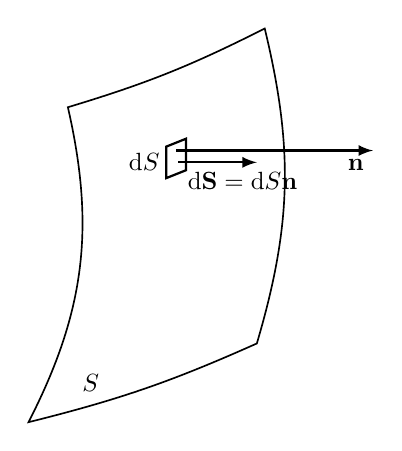
\begin{tikzpicture}[every node/.style={scale=.9}]
  \draw[semithick] (0,0) 
    to[bend right=20] ++(.5,4) 
    to[bend right=5] ++(2.5,1) 
    to[bend left=15] ++(-.1,-4) 
    to[bend left=5] node[pos=.75,above=2pt] {$S$} (0,0) --cycle;
  \draw[thick] (1.75,3.5) 
    node[below left=-1pt] {$\d S$} 
    --++(.25,.1) 
    --++(0,-.4) 
    node[below right=-3pt] {$\d \mathbf{S} = \d S\mathbf{n}$} 
    --++(-.25,-.1) --cycle;
  \draw[thick,-latex] (1.9,3.3) --++(1,0);
  \draw[thick,-latex] (1.875,3.45) --++(2.5,0) 
    node[below left] {$\mathbf{n}$};
\end{tikzpicture}
\end{document}